\chapter{Function Delivery Network}\label{chapter:FDN}

\section{General Aspects}
Current FaaS platforms are restricted to homogeneous clusters and serverless functions, which is a significant limitation due to the fact that heterogeneity of compute clusters and computational resources is steadily increasing in today's cloud applications. For instance, an IoT application may utilize an IoT cloud that consists of a cluster of multiple microcontroller-based systems, which might use different processor architectures and substantially differ in their hardware equipment, and another cluster composed of powerful Virtual Machines (VMs), which is responsible for handling the computationally more intensive tasks. Consequently, serverless functions that demand a significant amount of compute and data resources should be scheduled in an appropriate cluster that is able to fulfill these requirements. Additionally, it is important to mention that, due to hardware constraints present on edge devices, it can not be guaranteed that a certain FaaS platform can actually run on them, which prevents the use of a homogeneous FaaS platform over multiple heterogeneous clusters ~\parencite{fdn}. In summary, this implies the need for the possibility to deploy heterogeneous FaaS platforms in heterogeneous clusters and to schedule the execution of serverless functions based on their individual resource requirements. Simultaneously, data access behavior such as access latency should be taken into account in an effective manner in order to optimally utilize the available resources.

The Function Delivery Network (FDN) is a distributed network of target platforms, which is designed to extend the concept of serverless computing based on FaaS in order to overcome the mentioned limitations. It is highly versatile as it can be connected with a wide range of different target platforms due to the fact that it integrates with clusters that are dedicated for a multitude of purposes such as Cloud-, Edge- and High Performance Computing. Additionally, the FDN supports multiple FaaS providers like Apache OpenWhisk, OpenFaaS, AWS Lambda or Google Cloud Functions. 

\begin{figure}[H]
    \centering
    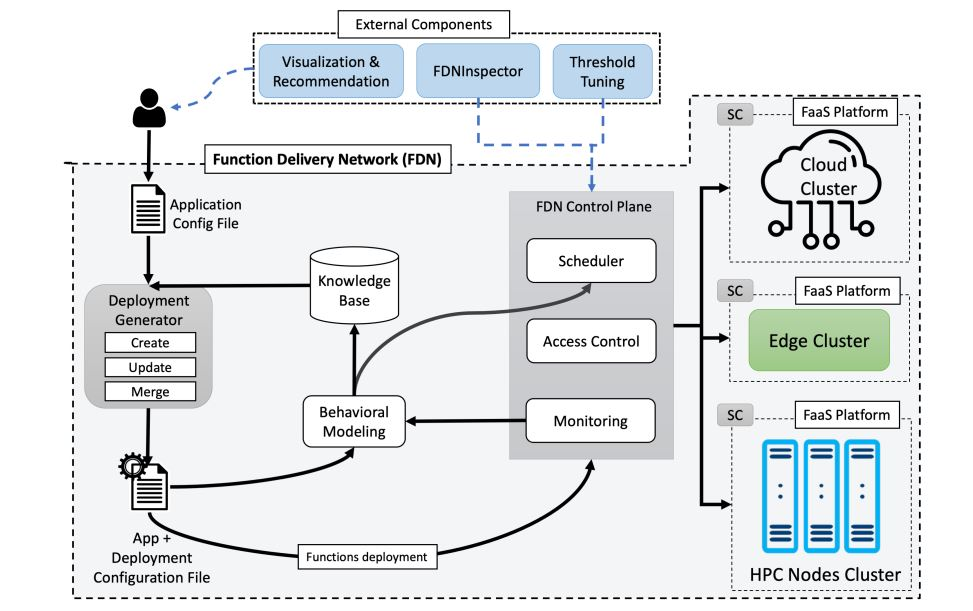
\includegraphics[width=1\textwidth]{./figures/fdn}
    \caption{Architecture of the Function Delivery Network}
    \label{fig:fdn}
\end{figure}

Figure \ref{fig:fdn} illustrates the general architectural and functional design of the FDN. The FDN realises the concept of FDaaS by requiring the user to submit an application configuration file, which describes the individual functions, APIs, permissions and other associated configuration. This file is subsequently passed to the following core components of the FDN:

\begin{enumerate}
    \item \textit{Deployment Generator}: This unit annotates the file with a deployment configuration for the specific application based on knowledge that was either previously collected by the FDN or externally provided by an expert.
    \item \textit{Control Plane}: This is the main component of the FDN. It is responsible for managing the access control which includes authentication and authorization as well as for monitoring the overall infrastructure and applications. Additionally, it handles data placement and the scheduling of function invocations based on the annotated deployment specification.
\end{enumerate}

The decisions that are made by the Control Plane at runtime regarding function scheduling and data placement depend on several behavioral models, which are created during the execution of an application by another component called \textit{Behavioral Modeling}. These models are continuously updated in an online learning fashion by extracting knowledge from data that is regularly collected by the FDN from the application's functions~\parencite{fdn}.

The various serverless clusters that are part of the Function Delivery Network are managed by a separate Kubernetes cluster composed of \textit{virtual kubelets}, which is an Open Source implementation of the Kubernetes kubelet that masquerades as a kubelet in order to connect Kubernetes with third-party APIs such as serverless container platforms (e. g. Azure Container Instances)~\parencite{virtual-kubelet}. The FDN employs a customized virtual kubelet which acts as a proxy service for a specific underlying serverless compute cluster that processes \usemintedstyle{bw}\mintinline{shell-session}|kubectl| commands in order to create and delete serverless functions inside the respective serverless cluster. Figure \ref{fig:fdn-vkubelet-provider} illustrates how the FDN employs virtual kubelets in order to manage its various target platforms and how they serve as an interface for external components.

\begin{figure}[H]
    \centering
    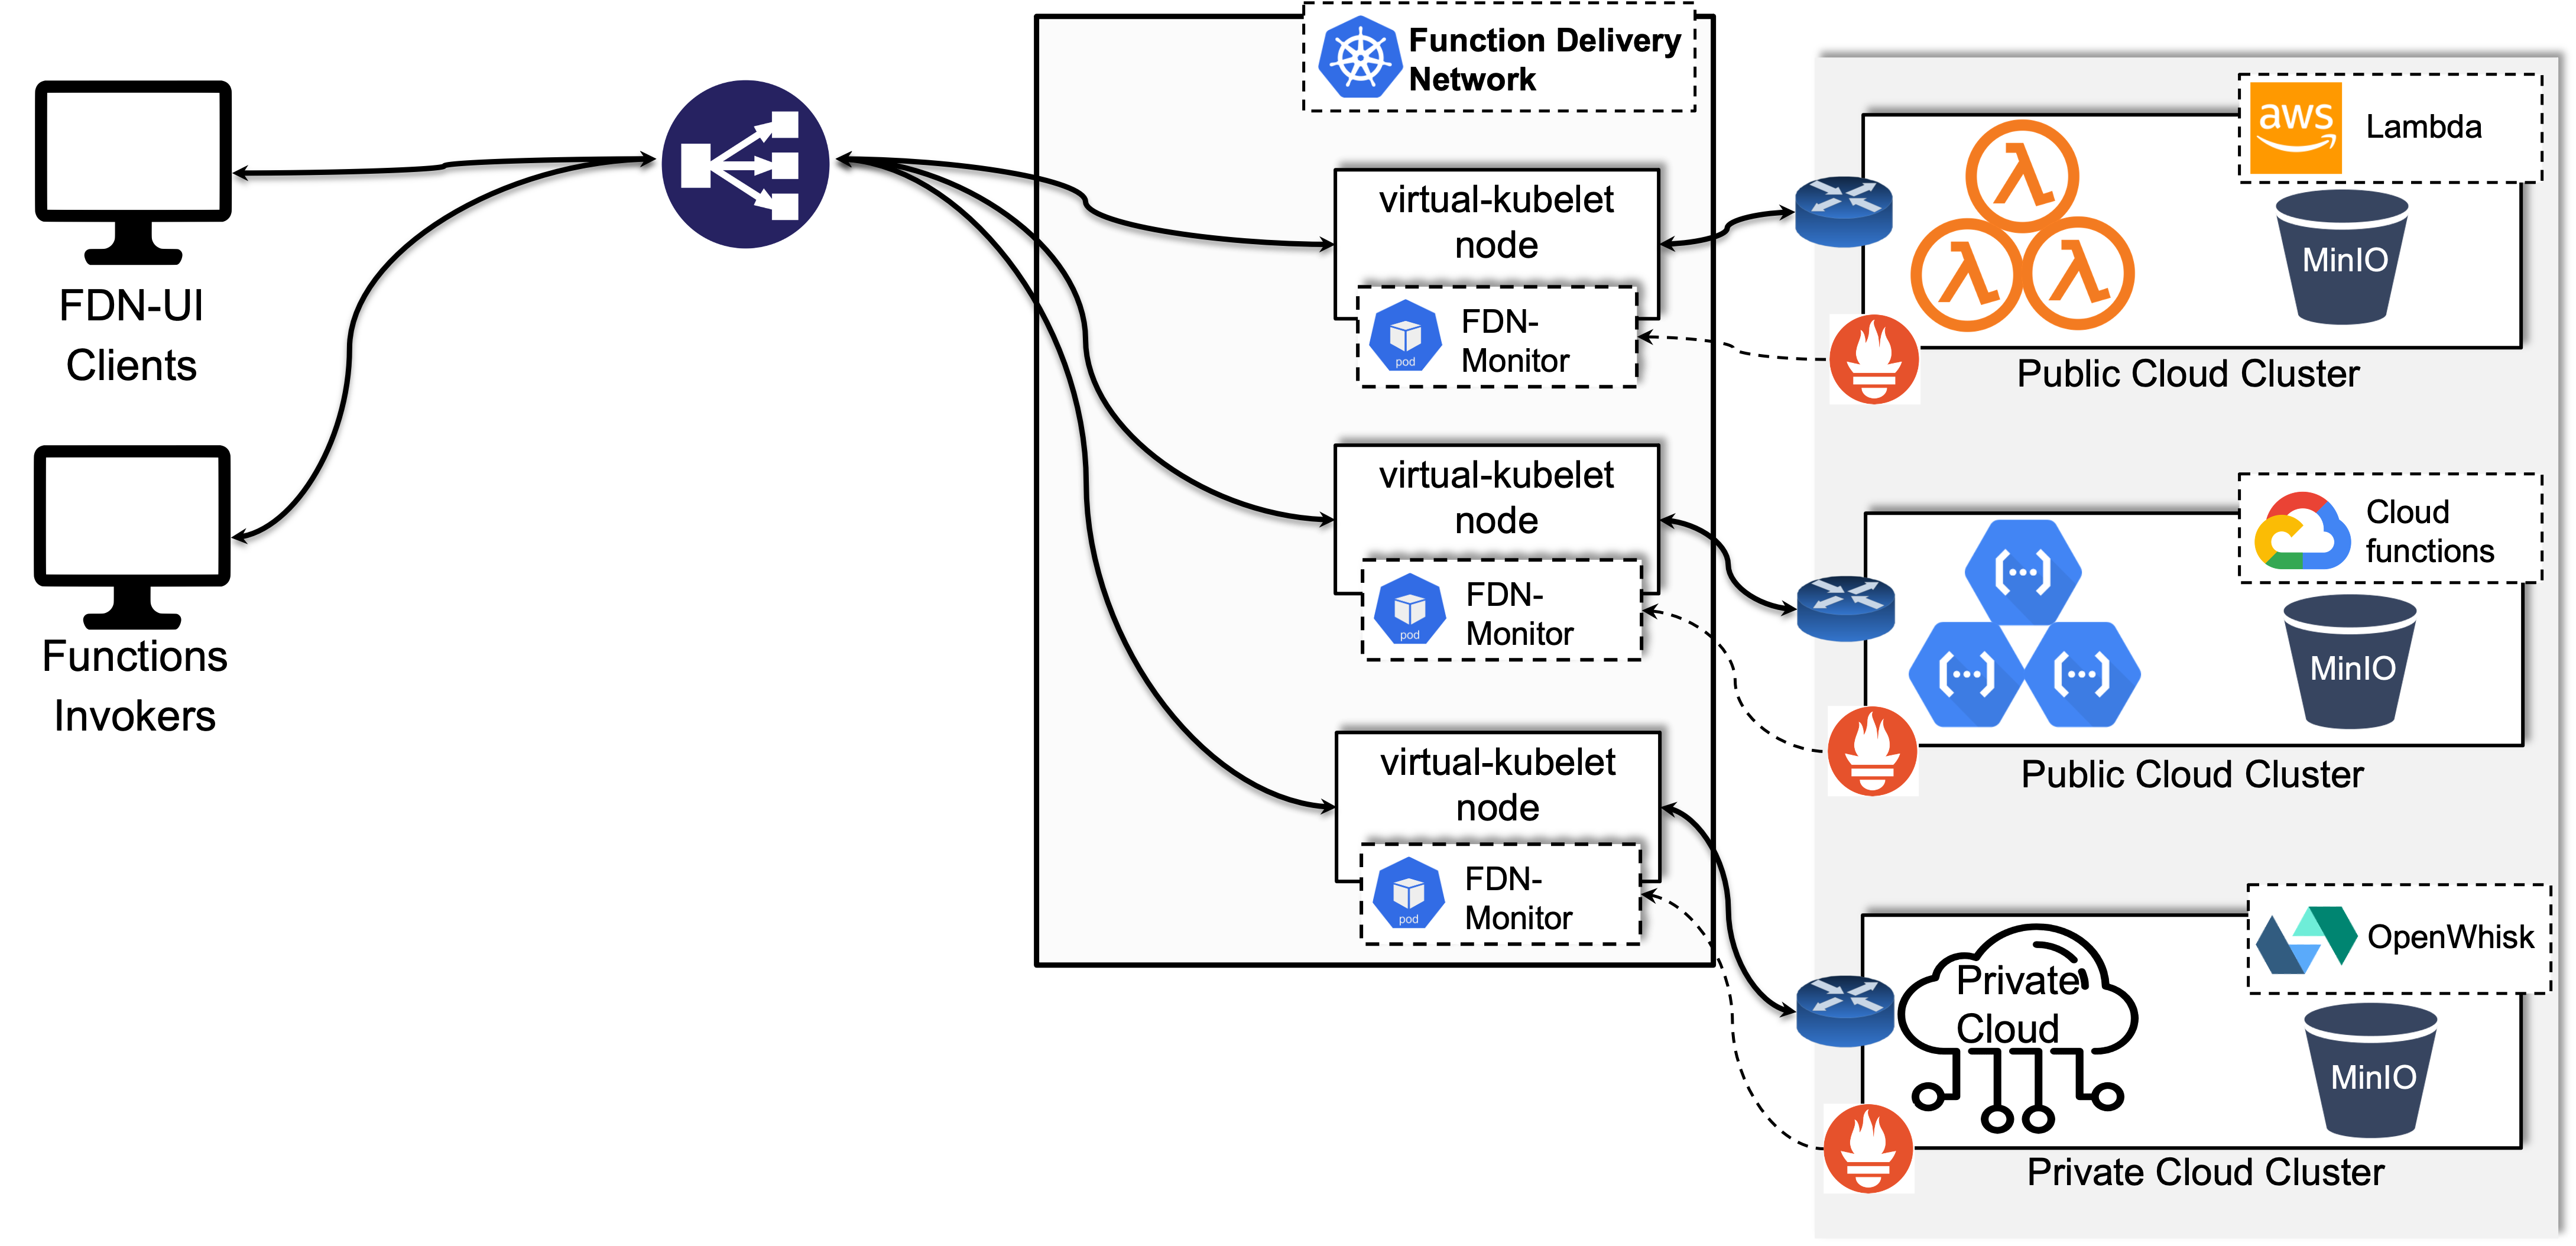
\includegraphics[width=1\textwidth]{./figures/fdn-vkubelet-provider}
    \caption{Virtual Kubelets operated by Function Delivery Network}
    \label{fig:fdn-vkubelet-provider}
\end{figure}


\section{Monitoring}
In order to monitor the various serverless clusters that are part of the Function Delivery Network, a comprehensive monitoring stack based on Prometheus, which is composed of a series of Kubernetes manifests, is installed to each of the operated clusters by applying the configuration using  \usemintedstyle{bw}\mintinline{shell-session}|kubectl|. Next to Grafana and Prometheus, the employed monitoring stack deploys the following components:

\begin{itemize}
    \item \textit{Prometheus Operator}: Provides a Kubernetes-native deployment of Prometheus and a set of custom resource definitions which facilitate and automate its configuration.
    \item \textit{Alertmanager}: Takes care of the correct processing of the various alerts sent by the Prometheus server.
    \item \textit{Node Exporter}: Exposes several metrics related to the operating system and hardware of Linux-based systems. This application is deployed to each node of the underlying Kubernetes cluster.
    \item \textit{Prometheus Adapter for Kubernetes Metrics APIs}: Implementation of the Kubernetes Custom Metrics and Resource Metrics API, which enables Kubernetes to use arbitrary metrics for autoscaling.
    \item \textit{kube-state-metrics}: Generates metrics related to various Kubernetes objects such as Deployments, Nodes and Pods.
\end{itemize}

Additionally, the FDN employs a client-based agent named \textit{FDN-Monitor}, which is responsible for collecting the metrics of a specific serverless cluster. Subsequently, the obtained data is aggregated into an instance of the high-speed time series database \textit{InfluxDB}. As illustrated by Figure \ref{fig:fdn-vkubelet-provider}, the FDN-Monitor is deployed as a sidecar container next to the virtual kubelets of the respective serverless clusters. The FDN-Monitor offers to collect the data from up to two Prometheus instances per cluster, which allows for a separate monitoring of the employed serverless platform (e.g. OpenFaaS) and the actual Kubernetes cluster. Ultimately, the data collected from the individual clusters is visualized by Grafana, which is configured to use the InfluxDB instance as underlying datasource. Additionally, in order to provide an appropriate visualization support, the FDN-Monitor supplies a set of preconfigured dashboards that can be imported in Grafana. 


\section{Experimental Edge Cluster}
In order to provide an answer to the question on how to implement and integrate individual power measurements for edge systems into the existing monitoring infrastructure of the FDN, an experimental edge cluster composed of a set of edge computers was established. The following sections aim on introducing the employed devices, how the cluster was technically set up and how it was integrated into the Function Delivery Network.

\subsection{Employed Edge Systems}
\subsubsection{Raspberry Pi 3 Model B v1.2}

\begin{figure}[h]
    \centering
    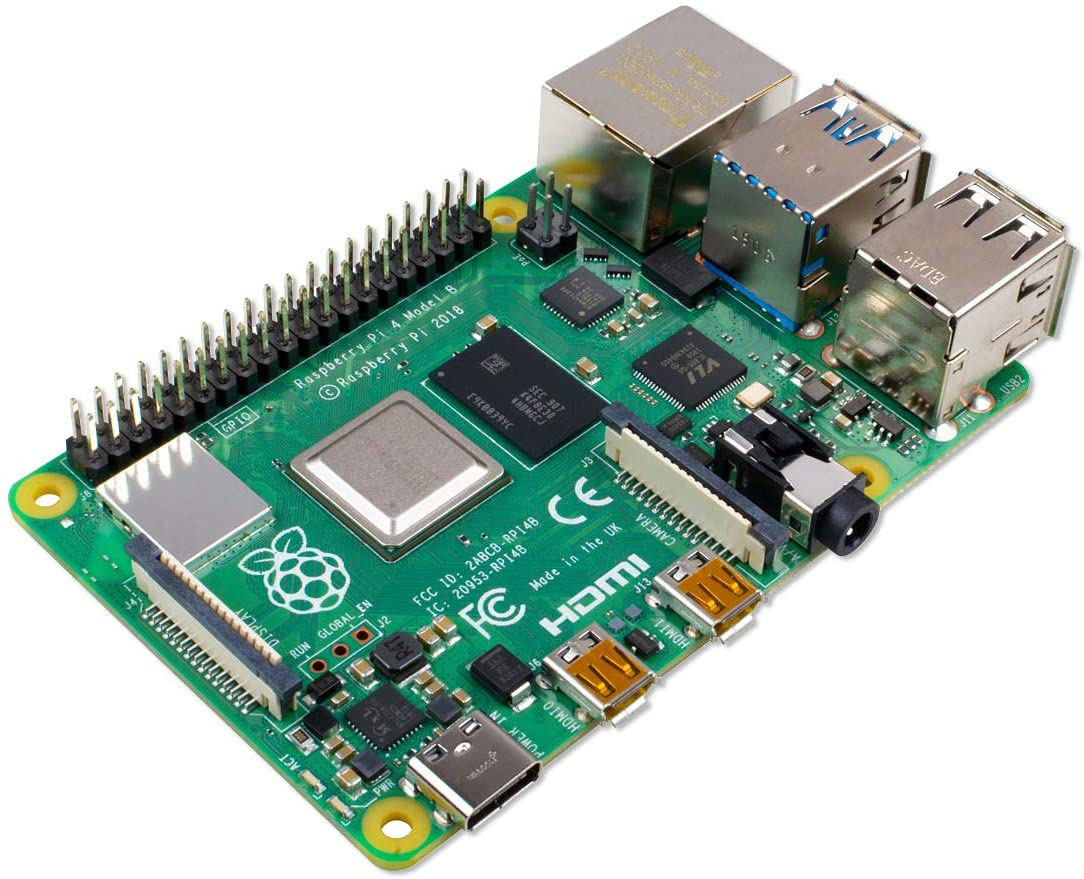
\includegraphics[width=0.30\textwidth]{./figures/mesh}
    \caption{Raspberry Pi 3 Model B v1.2}
    \label{fig:raspberry-pi}
\end{figure}


The Raspberry Pi 3 Model B v1.2 is the earliest model of the third generation of the Raspberry Pi, which is probably the most commonly known single-board computer in the world due to its affordability. It was developed by the british Raspberry Pi Foundation and is equipped with 1 GB of LPDDR2 RAM and a Cortex-A53 Quad-Core ARM64v8 processor with a Broadcom BCM2837 chipset that operates at 1.2 GHz. Even though the installed chip implements the 64-bit instruction set, the use of a 64-bit based operating system hardly offers a performance boost due to the low amount of available RAM which is why the Raspberry Pi used in this work runs a 32-bit Raspbian OS. In order to operate the Raspberry Pi a power supply of 5V at 2.5A via Micro-USB is required~\parencite{raspberry-pi-intro}.

\subsubsection{NVIDIA Jetson Nano Developer Kit}

\begin{figure}[h]
    \centering
    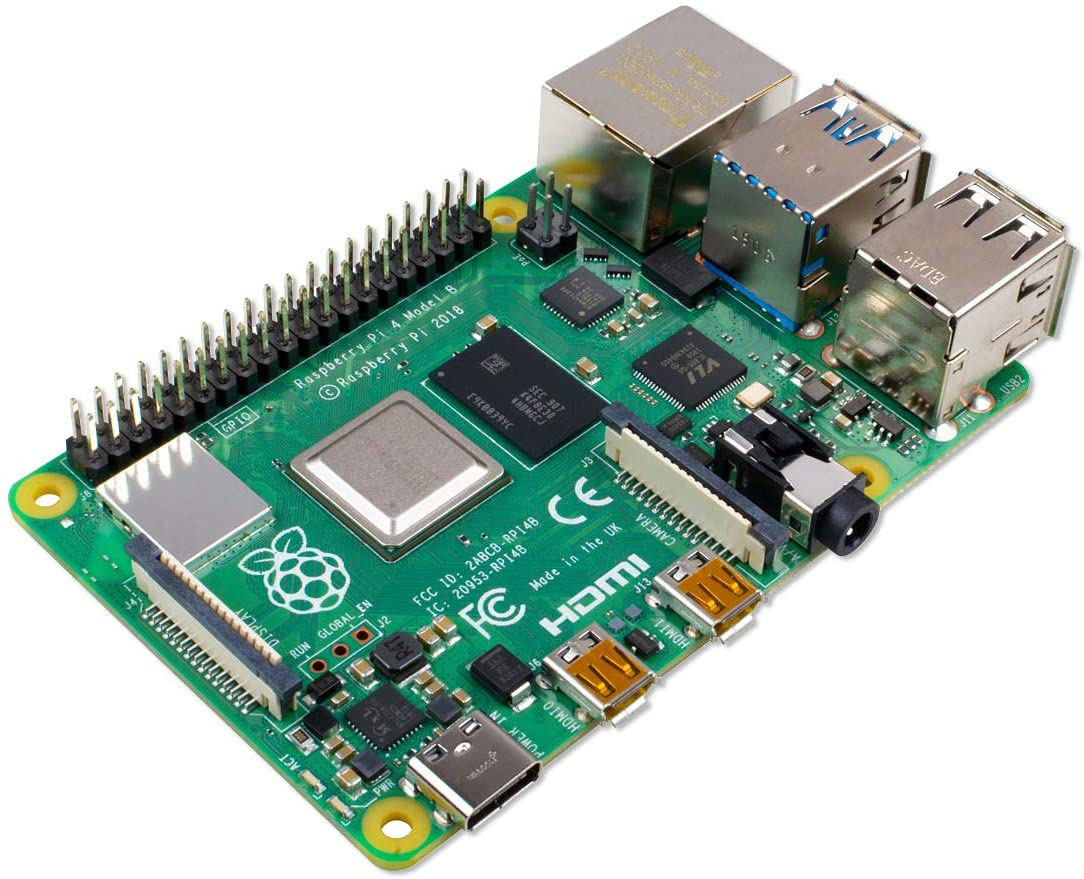
\includegraphics[width=0.30\textwidth]{./figures/mesh}
    \caption{NVIDIA Jetson Nano Developer Kit}
    \label{fig:jetson-nano}
\end{figure}

The NVIDIA Jetson Nano Developer Kit is a performant single-board computer developed by the NVIDIA Corporation and is primarily designed for the purpose of developing and executing AI applications. To this end, it is provided with a Cortex-A57 Quad-Core ARM64v8 CPU that runs at 1.43 GHz as well as with an NVIDIA 128-core NVIDIA Maxwell GPU. Additionally, the Jetson Nano Developer Kit has access to 4 GB of LPDDR4 RAM and requires a slightly higher power supply of 5V at 2.5A - however, supplying up to 4A is recommended.~\parencite{jetson-nano-devkit-manual}

\subsubsection{Google Coral Dev Board}

\begin{figure}[h]
    \centering
    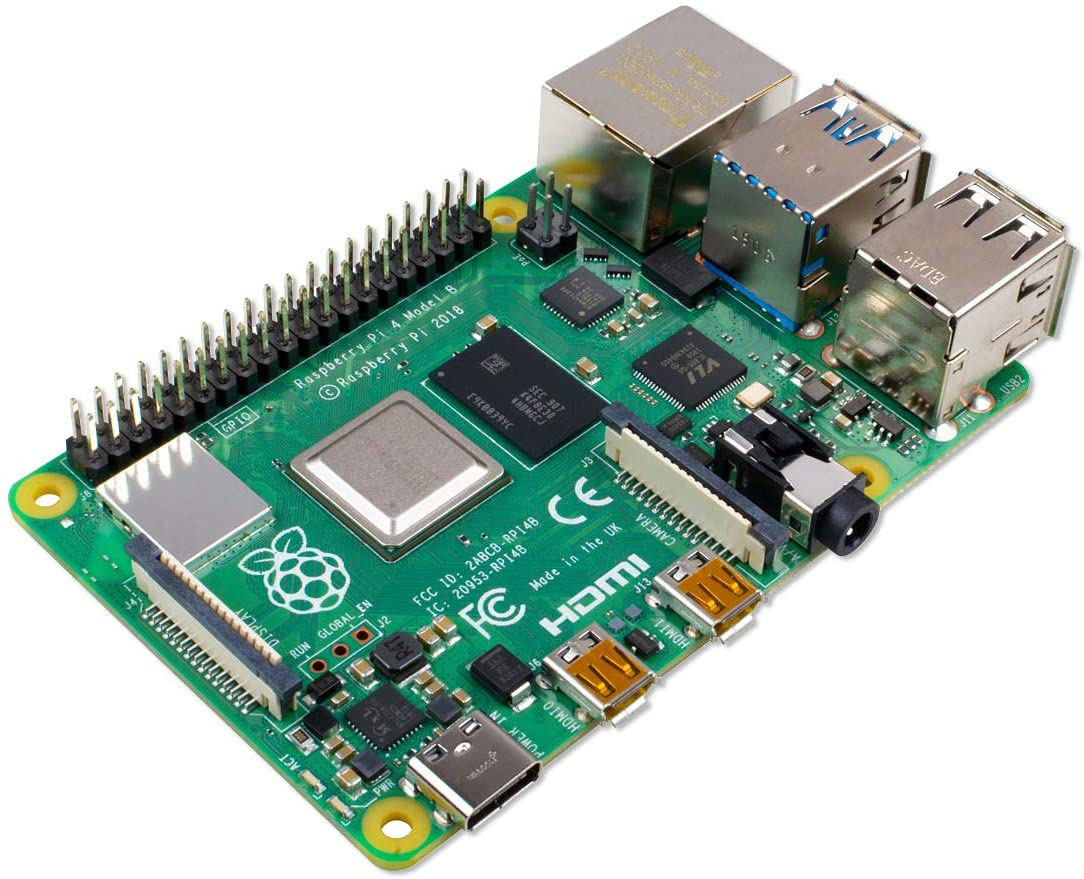
\includegraphics[width=0.30\textwidth]{./figures/mesh}
    \caption{Google Coral Dev Board}
    \label{fig:coral-dev-board}
\end{figure}

The Coral Dev Board is a single-board computer designed to facilitate machine learning inference and embedded system development. Next to a Vivante GC7000Lite GPU and a Cortex-A53 Quad-Core ARM64v8 processor that operates at up to 1.5 GHz, it is equipped with an Edge TPU coprocessor developed by Google which significantly leverages the performance. Moreover, it is provided with 1 GB of LPDDR4 RAM and demands a power supply of 5V at around 2-3A.~\parencite{coral-dev-board-manual}

\subsubsection{ODROID-XU4}

\begin{figure}[h]
    \centering
    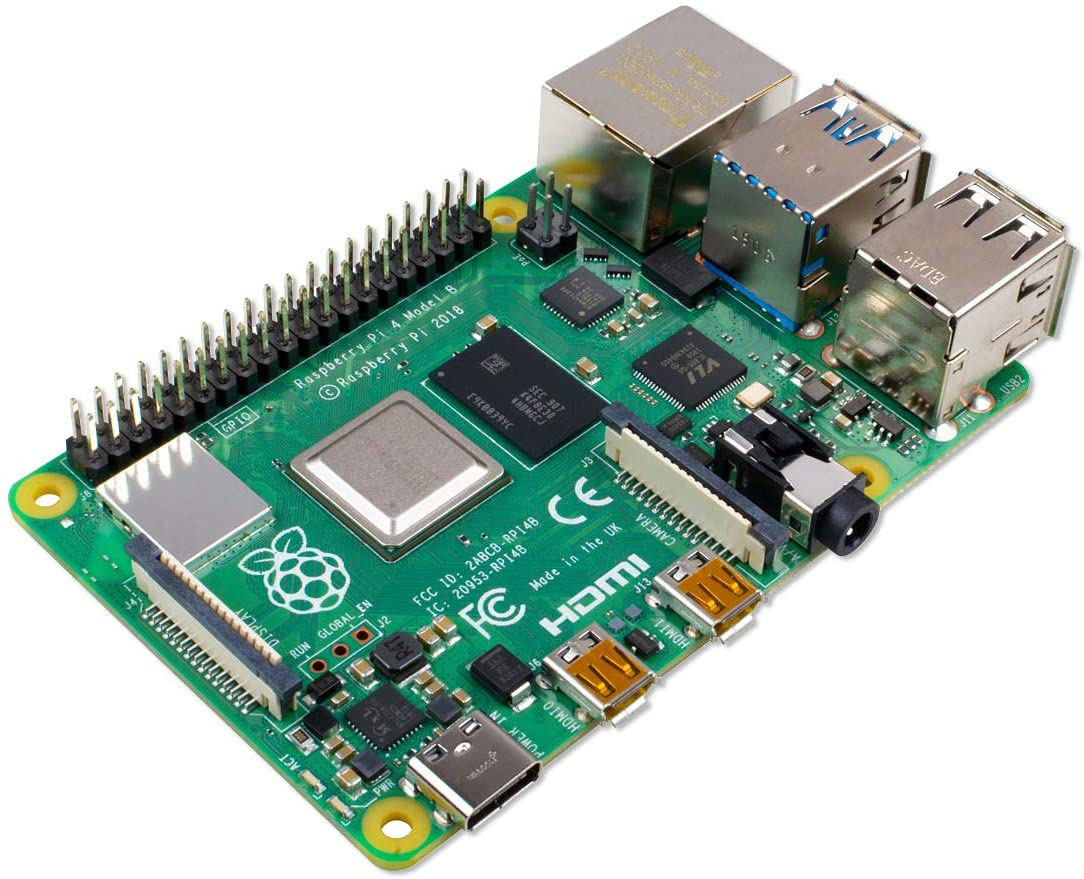
\includegraphics[width=0.30\textwidth]{./figures/mesh}
    \caption{ODROID-XU4}
    \label{fig:odroid-xu4}
\end{figure}

The ODROID-XU4 is a powerful single-board computer manufactured by Hardkernel, which is specifically well suited for developing software designed for the Android operating system. It comes with a SAMSUNG Exynos 5422 Octa-Core ARM32v7 CPU running at 2 GHz, an integrated Mali-T628MP6 GPU and 2 GB of LPDDR3 RAM. Even though the board consumes less than 1A in most of the cases, providing a power source supplying 5V at 4A is recommended in order to operate the XU4.~\parencite{odroid-xu4-manual}

\subsubsection{XILINX PYNQ-Z1}

\begin{figure}[h]
    \centering
    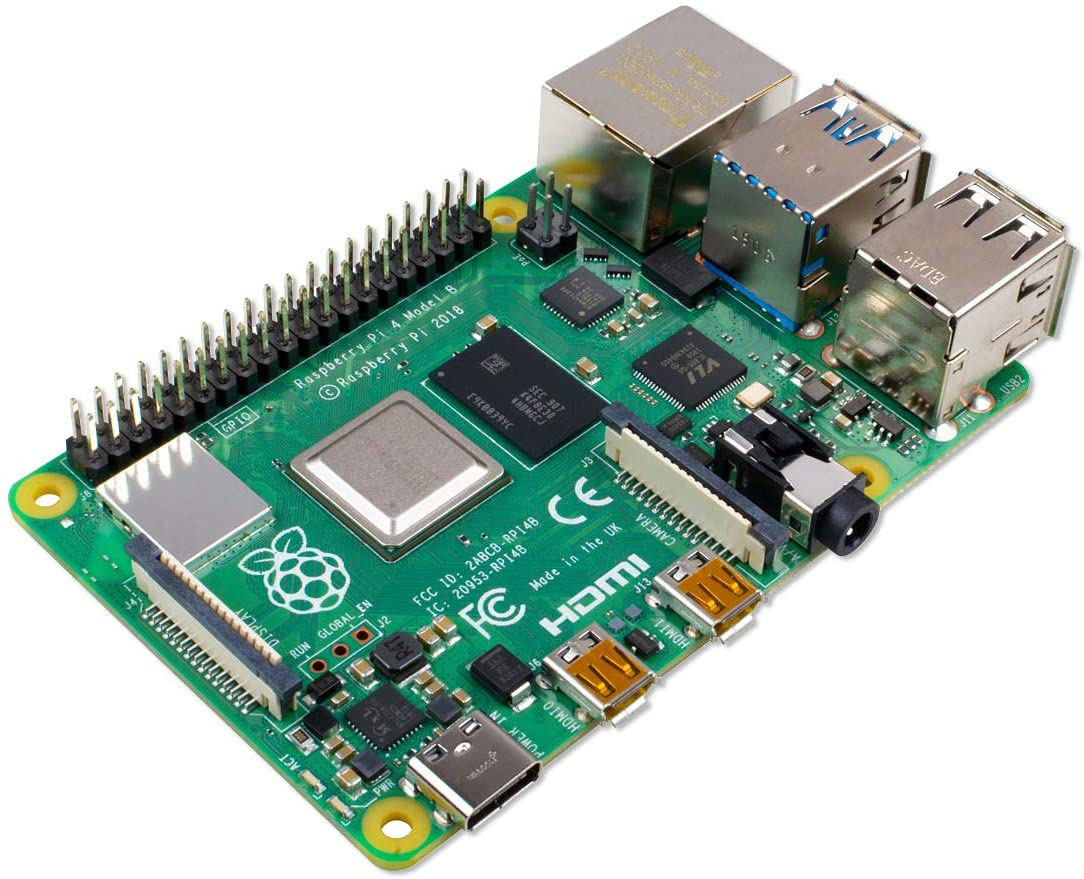
\includegraphics[width=0.30\textwidth]{./figures/mesh}
    \caption{XILINX PYNQ-Z1}
    \label{fig:xilinx-pynq-z1}
\end{figure}

The XILINX PYNQ-Z1 is a general purpose single-board computer manufactured by Digilent. It is designed to be used with the Open-Source framework PYNQ, which is based on the programming language Python and facilitates prototyping and embedded software development for the individual XILINX platforms. The board is supplied with 512MB of DDR3 RAM and a Cortex-A9 Dual-Core ARM32v7 processor which operates at up to 650 MHz. At the bare minimum, the PYNQ-Z1 can be powered via USB 2.0, which, according to the specifications, is able to provide 5V at up to 0.5A. For more complex applications, an external source supplying 7V at the minimum and 15V at the maximum should be used~\parencite{pynq-z1-manual}.

\subsection{Technical Establishment \& Integration}
The experimental edge cluster was set up using \textit{k3s}, which is a lightweight distribution of Kubernetes primarily designed for edge computing and IoT applications. Due to its compatibility with ARMv7- and ARM64-based devices it offers the possibility to establish a Kubernetes cluster composed of multiple heterogeneous edge computers and is thus perfectly suitable for the purpose of this work. Additionally, k3s does not place great demands on the hardware equipment which is why it can be deployed to a wide range of different devices, even to those with strictly limited resources~\parencite{k3s}. Consequently, after installing the necessities such as Docker and k3s on the individual machines, the edge cluster was initialized on the master node before adding each remaining system sequentially to the cluster by running the k3s agent using the previously obtained token required to perform a join. The individual nodes of the resulting cluster as well as their assigned names within Kubernetes and the cluster role that they fulfilled are outlined by Table \ref{table:cluster-topology}.

\begin{center}
\begin{table}[H]
\centering
\begin{tabular}{| c | c | c |} 
 \hline
 System & Node Name & Cluster Role \\ [0.5ex] 
 \hline\hline
 Linux Virtual Machine No. 1 & \usemintedstyle{bw}\mintinline[breaklines, breakafter=_]{shell-session}|vmschulz43| & Master \\ 
 \hline
 Linux Virtual Machine No. 2 & \usemintedstyle{bw}\mintinline[breaklines, breakafter=_]{shell-session}|vmschulz55| & Worker \\ 
 \hline
 Raspberry Pi 3 Model B v1.2 & \usemintedstyle{bw}\mintinline[breaklines, breakafter=_]{shell-session}|raspberrypi| & Worker \\ 
 \hline
 PYNQ-Z1 & \usemintedstyle{bw}\mintinline[breaklines, breakafter=_]{shell-session}|pynq| & Worker \\
 \hline
 ODROID-XU4 & \usemintedstyle{bw}\mintinline[breaklines, breakafter=_]{shell-session}|odroidxu4-1| & Worker \\
 \hline
 ODROID-XU4 Shifter Shield & \usemintedstyle{bw}\mintinline[breaklines, breakafter=_]{shell-session}|odroidxu4-2| & Worker \\
 \hline
 Google Coral Dev Board & \usemintedstyle{bw}\mintinline[breaklines, breakafter=_]{shell-session}|orange-finch| & Worker \\
 \hline
 NVIDIA Jetson Nano Developer Kit & \usemintedstyle{bw}\mintinline[breaklines, breakafter=_]{shell-session}|jetson-nano| & Worker \\ [1ex] 
 \hline
\end{tabular}
\caption{Topology of the experimental Kubernetes Edge Cluster}
\label{table:cluster-topology}
\end{table}
\end{center}

After successfully setting up the edge cluster with the help of Kubernetes, the next step was to install a corresponding serverless platform. Due to its natural integration with Kubernetes and its sophisticated UI, OpenFaaS was chosen as the employed serverless framework of the underlying edge cluster.

Subsequently, the monitoring infrastructure of the edge cluster had to be established. In the case of a cluster composed of resource-constrained nodes equipped with a rather limited amount of CPU cores and main memory, applying a extensive monitoring stack to a Kubernetes cluster takes up a large part of the available resources because of the numerous containers that are deployed for that purpose. Therefore, instead of spreading the monitoring workload across the edge devices, the associated containers were deployed to two virtual machines (VM) \usemintedstyle{bw}\mintinline[breaklines, breakafter=_]{shell-session}|vmschulz43| and \usemintedstyle{bw}\mintinline[breaklines, breakafter=_]{shell-session}|vmschulz55| which were also added to the cluster. Additionally, one of the VMs was assigned the role of the master node of the cluster since master nodes usually have to meet higher requirements in terms of available hardware resources. As a result, a significant amount of the resource-related burden induced by Kubernetes and the employed cluster monitoring stack was shifted away to the virtual machines which saved the precious resources on the edge devices that were needed for the execution of the various serverless functions.

Finally, the edge cluster was integrated into the Function Delivery Network by deploying a corresponding virtual kubelet in combination with an instance of the FDN-Monitor to the management cluster of the FDN.
